%%
%% This is file `mcmthesis-demo.tex',
%% generated with the docstrip utility.
%%
%% The original source files were:
%%
%% mcmthesis.dtx  (with options: `demo')
%%
%% -----------------------------------
%%
%% This is a generated file.
%%
%% Copyright (C)
%%       2010 -- 2015 by Zhaoli Wang
%%       2014 -- 2019 by Liam Huang
%%       2019 -- present by latexstudio.net
%%
%% This work may be distributed and/or modified under the
%% conditions of the LaTeX Project Public License, either version 1.3
%% of this license or (at your option) any later version.
%% The latest version of this license is in
%%   http://www.latex-project.org/lppl.txt
%% and version 1.3 or later is part of all distributions of LaTeX
%% version 2005/12/01 or later.
%%
%% This work has the LPPL maintenance status `maintained'.
%%
%% The Current Maintainer of this work is Liam Huang.
%%
%%
%% This is file `mcmthesis-demo.tex',
%% generated with the docstrip utility.
%%
%% The original source files were:
%%
%% mcmthesis.dtx  (with options: `demo')
%%
%% -----------------------------------
%%
%% This is a generated file.
%%
%% Copyright (C)
%%       2010 -- 2015 by Zhaoli Wang
%%       2014 -- 2019 by Liam Huang
%%       2019 -- present by latexstudio.net
%%
%% This work may be distributed and/or modified under the
%% conditions of the LaTeX Project Public License, either version 1.3
%% of this license or (at your option) any later version.
%% The latest version of this license is in
%%   http://www.latex-project.org/lppl.txt
%% and version 1.3 or later is part of all distributions of LaTeX
%% version 2005/12/01 or later.
%%
%% This work has the LPPL maintenance status `maintained'.
%%
%% The Current Maintainer of this work is Liam Huang.
%%
\documentclass{mcmthesis}
\mcmsetup{CTeX = false,    % 使用 CTeX 套装时,设置为 true
          tcn = {0000000}, problem = \textcolor{red}{A},
          sheet = true, titleinsheet = true, keywordsinsheet = true,
          titlepage = false, abstract = false}
		
\usepackage{newtxtext}	%Palatino的字体宏包
\usepackage[style=apa,backend=biber]{biblatex}	%参考文献排版引擎
\addbibresource{test_reference.bib}	%添加参考文献数据库

\usepackage{tocloft}	%修改目录 ,,,,
\setlength{\cftbeforesecskip}{6pt}	%设置章节标题在目录里的垂直距离
\renewcommand{\contentsname}{\hspace*{\fill}\Large\bfseries Contents \hspace*{\fill}}	%修改目录标题显示方式{\控制标题文本}{\水平居中}\大号字体\粗体

\title{Enjoy a Cozy and Green Bath}
% \author{\small \href{http://www.latexstudio.net/} 定义作者
%   {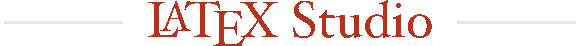
\includegraphics[width=7cm]{mcmthesis-logo}}}	在链接中嵌入一张图片
\date{\today}

\begin{document}

\begin{abstract}

Abstract part

\begin{keywords}
Keyword1, Keyword2, Keyword3, Keyword4
\end{keywords}

\end{abstract}

\maketitle

%% Generate the Table of Contents, if it's needed.
% \renewcommand{\contentsname}{\centering Contents}	居中显示
\tableofcontents        % 自动生成目录条目
\thispagestyle{empty}	%将目录页面设置为 empty 风格,意味着该页没有页眉和页脚
\newpage

\section{Introduction}

\subsection{Background}

Background Part

\subsection{Literature Review}

%Literature Review part	%参考文献的引用
%According to \textcite{kite2006}, 
%To address this, we introduce heat transfer formulas as 
%discussed (\cite[123]{man2002}). %123页

\subsection{Restatement of the Problem}

Restatement Part

In order to solve those problems, we will proceed as follows:

\begin{itemize}     %逐条列出
\item {\bf Stating assumptions}. By stating our assumptions, we will narrow the 
focus of our approach towards the problems and provide some insight into bathtub 
water temperature issues.
    
\item {\bf Making notations}. We will give some notations which are important for 
us to clarify our models.
    
\item {\bf Presenting our model}. In order to investigate the problem deeper, we 
divide our model into two sub-models. One is a steady convection heat transfer 
sub-model in which hot water is added constantly. The other one is an unsteady 
convection heat transfer sub-model where hot water is added discontinuously.

\item{\bf Defining evaluation criteria and conparing sub-models}.We define two 
main critia to 

\begin{itemize}
\item[1)] ... 
\item[2)] ...
\item[3)] ...
\item[4)] ...
\end{itemize}
    
\end{itemize}

\section{Assumptions and Justification}
To simplify the problem and make it convenient for us to simulate real-life 
conditions, we make the following basic assumptions, each of which is properly 
justified.

\begin{itemize}
\item {\bf The bath water is incompressible Non-Newtonian fluid}. The 
incompressible Non-Newtonian fluid is the basis of Navier–Stokes equations 
which are introduced to simulate the flow of bath water.
    
\item {\bf We ignore radiative thermal exchange}. According to Stefan-Boltzmann’s 
law, the radiative thermal exchange can be ignored when the temperature is low. 
Refer to industrial standard, the temperature in bathroom is lower than 
100 $^{\circ}$C, so it is reasonable for us to make this assumption.
    
\item {\bf The temperature of the adding hot water from the faucet is stable}. 
This hypothesis can be easily achieved in reality and will simplify our process 
of solving the problem.
\end{itemize}

\section{Notations}
\begin{center}           %将表格居中显示
\begin{tabular}{clc}     %将表格分为三列 居中 左对齐 居中
{\bf Symbols} & {\bf description} & \quad {\bf Unit} \\[0.25cm]    %表头 \quad分隔符  \\[0.25cm] 标题与下一行的距离
$h$ & Convection heat transfer coefficient & \quad W/(m$^2 \cdot$ K) 
\\[0.2cm]
$k$ & Thermal conductivity & \quad W/(m $\cdot$ K) \\[0.2cm]
$c_p$ & Specific heat & \quad J/(kg $\cdot$ K) \\[0.2cm]
$\Theta$ & Density & \quad kg/m$^2$ \\[0.2cm]
$\delta$ & Thickness & \quad m \\[0.2cm]
$t$ & Temperature & \quad $^\circ$C, K \\[0.2cm]
$\tau$ & Time & \quad s, min, h \\[0.2cm]
$q_m$ & Mass flow & \quad kg/s \\[0.2cm]
$\Phi$ & Heat transfer power & \quad W \\[0.2cm]
$T$ & A period of time & \quad s, min, h \\[0.2cm]
$V$ & Volume & \quad m$^3$, L \\[0.2cm]
$M,\,m$ & Mass & \quad kg \\[0.2cm]
$A$ & Aera & \quad m$^2$ \\[0.2cm]
$a,\,b,\,c$ & The size of a bathtub  & \quad m$^3$  %,\,添加小间距
\end{tabular}
\end{center}

\noindent where we define the main parameters while specific value of those 
parameters will be given later.

\section{Model Overview}
After deriving the value of parameters, we deduce formulas 
to derive results and simulate the change of temperature field via CFD, as 
described by \textcite{Dyson2006}.

\begin{figure}[h]   %定义图形环境 h:here、t:top、b:bpttem、p:单独一页放置浮动体
\centering          %水平居中
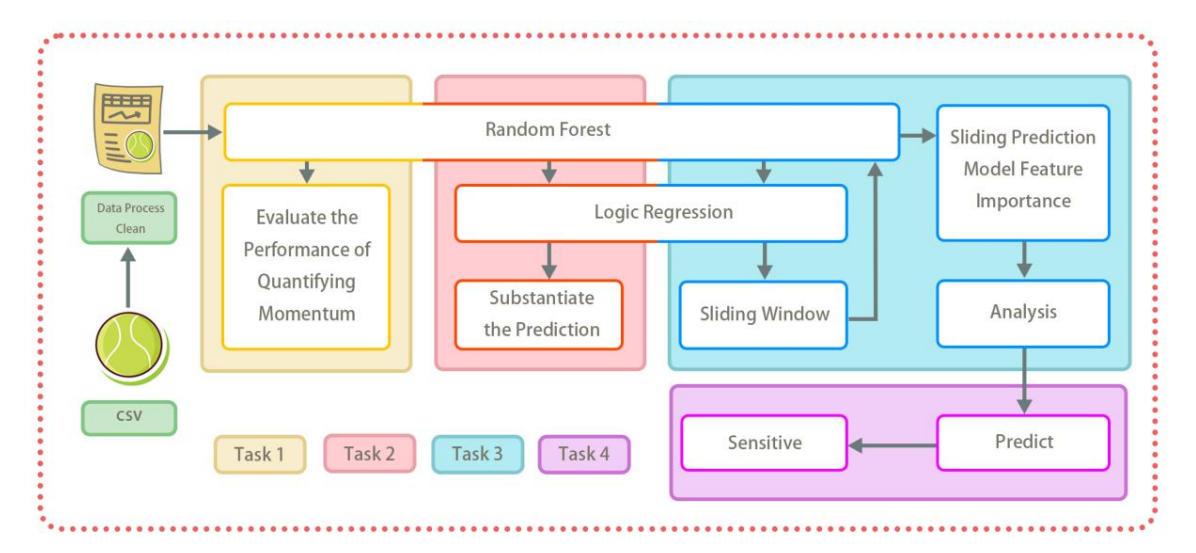
\includegraphics[width=12cm]{"C:/Users/admin/Desktop/GitHub/MCM/test/51XX/1.png"}
\caption{GoogleNet} \label{fig1}    %创建标签以便在文档中使用
\end{figure}

\section{Sub-model I : Adding Water Continuously}
Sub-model I 

\subsection{Model Establishment}
Model Establishment 

\subsubsection{Control Equations and Boundary Conditions}
We assume the hot water in the bathtub as a cube. Then we put it into a
rectangular coordinate system. The length, width, and height of it is $a,\, b$ 
and $c$.

%\begin{figure}[h] 
%\centering
%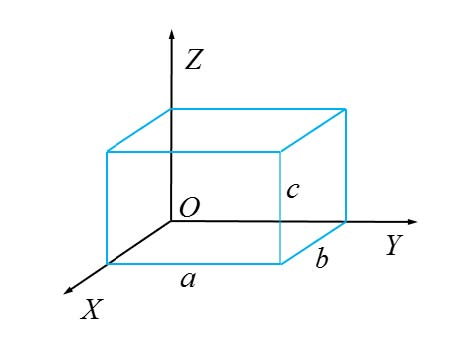
\includegraphics[width=8cm]{fig2.jpg}
%\caption{Modeling process} \label{fig2}
%\end{figure}

In the basis of this, we introduce the following equations:

\begin{itemize}
\item {\bf Continuity equation:}
\end{itemize}

\begin{equation} \label{eq1}        % 定义带编号的数学公式环境 为公式添加标签eq1 方便引用
\frac{\partial u}{\partial x} + \frac{\partial v}{\partial y} +
\frac{\partial w}{\partial z} = 0   % \frac 创建分数形式 \partial 求偏导
\end{equation}
    
\noindent where the first component is the change of fluid mass along the $X$-ray. 
The second component is the change of fluid mass along the $Y$-ray. And the third 
component is the change of fluid mass along the $Z$-ray. The sum of the change in 
mass along those three directions is zero.

\begin{itemize}
\item {\bf Moment differential equation (N-S equations):}
\end{itemize}

\begin{equation} \label{eq2}
    \left\{     %大括号
    \begin{array}{l} \!\!   %数组环境 用来对齐多个方程 \!\!减少公式间的间距 增加紧凑性
    \rho \Big(u \dfrac{\partial u}{\partial x} + v \dfrac{\partial u}{\partial y} + 
    w\dfrac{\partial u}{\partial z} \Big) = -\dfrac{\partial p}{\partial x} + 
    \eta \Big(\dfrac{\partial^2 u}{\partial x^2} + \dfrac{\partial^2 u}{\partial y^2} + 
    \dfrac{\partial^2 u}{\partial z^2} \Big) \\[0.3cm]
    \rho \Big(u \dfrac{\partial v}{\partial x} + v \dfrac{\partial v}{\partial y} + 
    w\dfrac{\partial v}{\partial z} \Big) = -\dfrac{\partial p}{\partial y} + 
    \eta \Big(\dfrac{\partial^2 v}{\partial x^2} + \dfrac{\partial^2 v}{\partial y^2} + 
    \dfrac{\partial^2 v}{\partial z^2} \Big) \\[0.3cm]
    \rho \Big(u \dfrac{\partial w}{\partial x} + v \dfrac{\partial w}{\partial y} +
    w\dfrac{\partial w}{\partial z} \Big) = -g-\dfrac{\partial p}{\partial z} + 
    \eta \Big(\dfrac{\partial^2 w}{\partial x^2} + \dfrac{\partial^2 w}{\partial y^2} + 
    \dfrac{\partial^2 w}{\partial z^2} \Big)  
    \end{array}
    \right.
    \end{equation}

\begin{itemize}
\item{\bf Energy differential equation:}
\end{itemize}

\begin{equation} \label{eq3}
\rho c_p \Big( u\frac{\partial t}{\partial x} + v\frac{\partial t}{\partial y} + 
w\frac{\partial t}{\partial z} \Big) = \lambda \Big(\frac{\partial^2 t}{\partial x^2} + 
\frac{\partial^2 t}{\partial y^2} + \frac{\partial^2 t}{\partial z^2} \Big)
\end{equation}

\noindent where the left three components are convection terms while the right 
three components are conduction terms.

By Equation \eqref{eq3}, we have ......

......

On the right surface in Fig. \ref{fig2}, the water also transfers heat firstly 
with bathtub inner surfaces and then the heat comes into air. The boundary 
condition here is ......

\subsubsection{Definition of the Mean Temperature}

......

\subsubsection{Determination of Heat Transfer Capacity}

......

\section{Sub-model II: Adding Water Discontinuously}

......

\subsection{Heating Model}

\subsubsection{Control Equations and Boundary Conditions}

\subsubsection{Determination of Inflow Time and Amount}

\subsection{Standby Model}

\subsection{Results}

\quad~ We first give the value of parameters based on others’ studies. Then we 
get the calculation results and simulating results via those data.
%quad:插入水平空间 创建标准空格
%~:非断行空格 确保两个元素在一行 

\subsubsection{Determination of Parameters}
.....

\subsubsection{Calculating Results}

Putting the above value of parameters into the equations we derived before, we 
can get the some data as follows:

%%普通表格
\begin{table}[h]  %h表示固定在当前位置
\centering        %设置居中
\caption{The calculating results}  %表标题
\vspace{0.15cm}     %垂直距离
\label{tab2}        %引用标签                  %设置表的引用标签
\begin{tabular}{|c|c|c|}  %3个c表示3列, |可选, 表示绘制各列间的竖线
\hline                    %画横线
Variables & Values & Unit     \\ \hline  %各列间用&隔开
$A_1$     & 1.05   &   $m^2$  \\ \hline
$A_2$     & 2.24   &   $m^2$  \\ \hline
$\Phi_1$  & 189.00 &   $W$   \\ \hline
$\Phi_2$  & 43.47  &   $W$   \\ \hline
$\Phi$    & 232.47 &   $W$   \\ \hline
$q_m$     & 0.014  &   $g/s$ \\ \hline
\end{tabular}
\end{table}
    
From Table \ref{tab2}, ......
    
......
    
\section{Correction and Contrast of Sub-Models}

......
    
\subsection{Correction with Evaporation Heat Transfer}
    
......
    
\subsection{Contrast of Two Sub-Models}
    
......
    
\section{Model Analysis and Sensitivity Analysis}
    
the shape and volume of 
the tub, the shape/volume/temperature/motions of the person, and the bubbles 
made from bubble bath additives, as discussed 
in (\cite{evaporation2018}; \cite{thesis2015}).
    
\subsection{The Influence of Different Bathtubs}
    
......
    
\subsubsection{Different Volumes of Bathtubs}
    
...

We assume the initial volume to be 280 L and change it by $\pm 5$\%, $\pm 8$\%, 
$\pm 12$\% and $\pm 15$\%. With the aid of sub-models we established before, the 
variation of some parameters turns out to be as follows

%%三线表
\begin{table}[h] %h表示固定在当前位置
\centering  %设置居中
\caption{Variation of some parameters}  %表标题
\label{tab7} %设置表的引用标签
\begin{tabular}{ccccccc} %7个c表示7列, c表示每列居中对齐, 还有l和r可选
\toprule  %画顶端横线
$V$      & $A_1$   & $A_2$   & $T_2$    & $q_{m1}$ & $q_{m2}$ & $\Phi_q$ \\     %定义表头*
\midrule  %画中间横线
-15.00\% & -5.06\% & -9.31\% & -12.67\% & -2.67\%  & -14.14\% & -5.80\% \\
-12.00\% & -4.04\% & -7.43\% & -10.09\% & -2.13\%  & -11.31\% & -4.63\% \\
-8.00\%  & -2.68\% & -4.94\% & -6.68\%  & -1.41\%  & -7.54\%  & -3.07\% \\
-8.00\%  & -2.68\% & -4.94\% & -6.68\%  & -1.41\%  & -7.54\%  & -3.07\% \\
-8.00\%  & -2.68\% & -4.94\% & -6.68\%  & -1.41\%  & -7.54\%  & -3.07\% \\
-8.00\%  & -2.68\% & -4.94\% & -6.68\%  & -1.41\%  & -7.54\%  & -3.07\% \\
-8.00\%  & -2.68\% & -4.94\% & -6.68\%  & -1.41\%  & -7.54\%  & -3.07\% \\
-8.00\%  & -2.68\% & -4.94\% & -6.68\%  & -1.41\%  & -7.54\%  & -3.07\% \\
-8.00\%  & -2.68\% & -4.94\% & -6.68\%  & -1.41\%  & -7.54\%  & -3.07\% \\
-8.00\%  & -2.68\% & -4.94\% & -6.68\%  & -1.41\%  & -7.54\%  & -3.07\% \\
-8.00\%  & -2.68\% & -4.94\% & -6.68\%  & -1.41\%  & -7.54\%  & -3.07\% \\
\bottomrule  %画底部横线
\end{tabular}
\end{table}

\section{Strength and Weakness}

\subsection{Strength}
    
\begin{itemize}
\item ...
    
\item ...
    
\item ...
    
\item ...
    
\end{itemize}
    
\subsection{Weakness}
    
\begin{itemize}
\item ...

\item ...
   
\item ...

\end{itemize}
    
\section{Further Discussion}
    
In addition, we make improvements for applying our model in real life, as suggested by the patent \textcite{patent2023}.
    

\begin{itemize}
\item Different Distribution of Inflow Faucets
    
In our before discussion, we assume there being just one entrance of inflow.
    
From the simulating outcome, we find the temperature of bath water is hardly even. 
So we come up with the idea of adding more entrances.
    
The simulation turns out to be as follows
    
%\begin{figure}[h] 
%\centering
%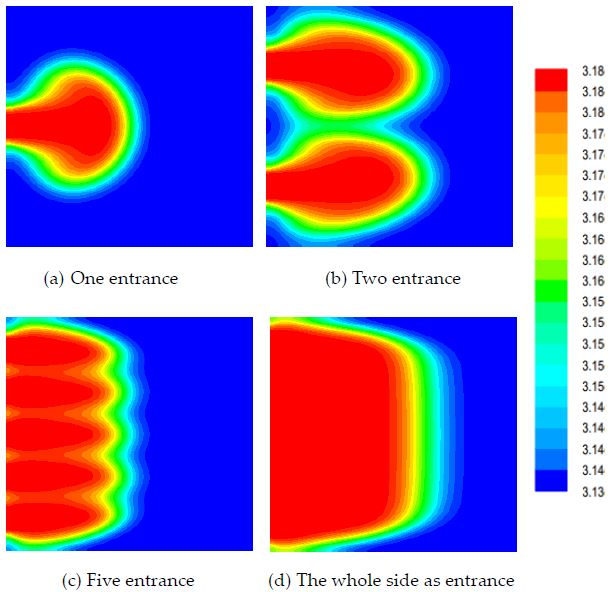
\includegraphics[width=12cm]{fig24.jpg}
%\caption{The simulation results of different ways of arranging entrances} \label{fig24}
%\end{figure}
    

In conclusion, if we design more entrances, it will be easier to realize the goal 
to keep temperature even throughout the bathtub.
    
\item Model Application
    
Our before discussion is based on ideal assumptions. In reality, we have to make 
some corrections and improvement.
    
\begin{itemize}
\item[1)] Adding hot water continually with the mass flow of 0.16 kg/s. This way 
can ensure even mean temperature throughout the bathtub and waste less water.
    
\item[2)] The manufacturers can design an intelligent control system to monitor 
the temperature so that users can get more enjoyable bath experience.
    
\item[3)] We recommend users to add bubble additives to slow down the water being 
cooler and help cleanse. The additives with lower thermal conductivity are optimal.
    
\item[4)] The study method of our establishing model can be applied in other area 
relative to convection heat transfer, such as air conditioners.
\end{itemize}
\end{itemize}
    
\printbibliography  %打印参考文献
    
\newpage
    
\begin{letter}{Enjoy Your Bath Time!}   %信息环境搭建
    
......
    
    
\begin{itemize}
\item Adding hot water consistently
\item Using smaller bathtub if possible
\item Decreasing motions during bath
\item Using bubble bath additives
\item Arranging more faucets of inflow
\end{itemize}
    
\vspace{\parskip}       %增加一个垂直间距
    
Sincerely yours,
    
Your friends
    
\end{letter}
    
\newpage
    
\begin{appendices}

\section{First appendix}

appendix1    
Here is simulation programme we used in our model as follow (\cite{Liu02}).\\

\textbf{\textcolor[rgb]{0.98,0.00,0.00}{Input matlab source:}}  %textbf加粗文本 
\lstinputlisting[language=Matlab]{./code/mcmthesis-matlab1.m}   %插入外部代码文件内容 [matlab语言]{路径}
    
\section{Second appendix}
    
some more text \textcolor[rgb]{0.98,0.00,0.00}{\textbf{Input C++ source:}}
\lstinputlisting[language=C++]{./code/mcmthesis-sudoku.cpp}
    
\end{appendices}
    
\newpage
\newcounter{lastpage}   
\setcounter{lastpage}{\value{page}} %分页处理时 记录当前页码
\thispagestyle{empty}   %去掉页眉页脚
    
\section*{Report on Use of AI}  %创建章节_关于使用人工智能的报告
    
\begin{enumerate}   %创建有序列表
\item OpenAI ChatGPT (Nov 5, 2023 version, ChatGPT-4,)  %列表第一项
\begin{description}     %第一项的介绍
\item[Query1:] <insert the exact wording you input into the AI tool> 
\item[Output:] <insert the complete output from the AI tool>
\end{description}
\item OpenAI Ernie (Nov 5, 2023 version, Ernie 4.0) 
\begin{description}
\item[Query1:] <insert the exact wording of any subsequent input into the AI tool> 
\item[Output:] <insert the complete output from the second query>
\end{description}
\item Github CoPilot (Feb 3, 2024 version) 
\begin{description}
\item[Query1:] <insert the exact wording you input into the AI tool> 
\item[Output:] <insert the complete output from the AI tool>
\end{description}
\item Google Bard (Feb 2, 2024 version) 
\begin{description}
\item[Query1:] <insert the exact wording of your query> 
\item[Output:] <insert the complete output from the AI tool>
\end{description}
\end{enumerate}
    
% 重置页码
\clearpage  %插入分页符
\setcounter{page}{\value{lastpage}}    
    
\end{document}
%%
%% This work consists of these files mcmthesis.dtx,
%%                                   figures/ and
%%                                   code/,
%% and the derived files             mcmthesis.cls,
%%                                   mcmthesis-demo.tex,
%%                                   README,
%%                                   LICENSE,
%%                                   mcmthesis.pdf and
%%                                   mcmthesis-demo.pdf.
%%
%% End of file `mcmthesis-demo.tex'.
    